% preamble-exam-zh.tex — 共享 preamble
% 用于所有 exam-zh 模板
%
% 样式策略：
%   屏幕 → 语义彩色（蓝=关键想法，红=易错，绿=路线，灰=提示/教师备注）
%   打印 → 自动降级为黑白（通过 print mode 或 monochrome 选项）

\documentclass{exam-zh}

% ---------- 基础配置 ----------
\examsetup{
  page/size = a4paper,
  page/show-head = false,
  page/show-foot = false,
  sealline/show = false,
  font = times,
  math-font = xits,
}

\usepackage{tcolorbox}
\usepackage{needspace}
\usepackage{graphicx}
\usepackage{tikz}
\usetikzlibrary{calc,arrows.meta,intersections}
\tcbuselibrary{skins,breakable}

% ---------- 打印/屏幕颜色切换 ----------
% 用法：\documentclass[monochrome]{exam-zh} 即可切换为纯黑白
% 注意：不要使用 \if@xxx 放在 makeatother 外部；这里改成普通条件名。
\newif\ifeduprintcolor
\eduprintcolortrue

\makeatletter
\@ifclasswith{exam-zh}{monochrome}{\eduprintcolorfalse}{}
\makeatother

% ---------- 语义颜色定义 ----------
% 屏幕：有色彩区分；打印：降级为灰度
\ifeduprintcolor
  % --- 屏幕彩色模式 ---
  \definecolor{edu-blue}{RGB}{47, 82, 122}       % 关键想法
  \definecolor{edu-blue-bg}{RGB}{243, 246, 252}
  \definecolor{edu-red}{RGB}{180, 40, 40}         % 易错提醒
  \definecolor{edu-red-bg}{RGB}{255, 245, 240}
  \definecolor{edu-green}{RGB}{34, 100, 60}       % 路线图
  \definecolor{edu-green-bg}{RGB}{242, 250, 245}
  \definecolor{edu-orange}{RGB}{160, 90, 0}       % 训练目标
  \definecolor{edu-orange-bg}{RGB}{255, 248, 235}
  \definecolor{edu-gray}{RGB}{100, 100, 100}      % 提示/教师备注
  \definecolor{edu-gray-bg}{RGB}{248, 248, 248}
  \definecolor{edu-purple}{RGB}{90, 50, 120}      % 思考题
  \definecolor{edu-purple-bg}{RGB}{248, 244, 252}
\else
  % --- 打印黑白模式 ---
  \definecolor{edu-blue}{gray}{0.15}
  \definecolor{edu-blue-bg}{gray}{0.96}
  \definecolor{edu-red}{gray}{0.25}
  \definecolor{edu-red-bg}{gray}{0.97}
  \definecolor{edu-green}{gray}{0.20}
  \definecolor{edu-green-bg}{gray}{0.97}
  \definecolor{edu-orange}{gray}{0.25}
  \definecolor{edu-orange-bg}{gray}{0.98}
  \definecolor{edu-gray}{gray}{0.40}
  \definecolor{edu-gray-bg}{gray}{0.97}
  \definecolor{edu-purple}{gray}{0.30}
  \definecolor{edu-purple-bg}{gray}{0.98}
\fi
\colorlet{edu-diagram-muted}{edu-gray}

% ---------- 自定义教学环境 ----------
% 共性：enhanced + breakable（跨页不断裂）

% 原题卡片 — 强边框，突出显示
\newtcolorbox{problemcard}{
  enhanced, breakable,
  colback=edu-blue-bg,
  colframe=edu-blue,
  boxrule=1.2pt,
  arc=0pt,
  left=3mm, right=3mm, top=3mm, bottom=3mm,
}

% 解题路线图 — 左边线 + 浅底
\newtcolorbox{routebox}{
  enhanced, breakable,
  colback=edu-green-bg,
  colframe=edu-green!30,
  boxrule=0pt,
  borderline west={2.5pt}{0pt}{edu-green},
  left=3mm, right=3mm, top=3mm, bottom=3mm,
}

% 关键想法 — 蓝色左边线
\newtcolorbox{keyideabox}{
  enhanced, breakable,
  colback=edu-blue-bg,
  colframe=edu-blue!30,
  boxrule=0pt,
  borderline west={2.5pt}{0pt}{edu-blue},
  left=3mm, right=3mm, top=3mm, bottom=3mm,
}

% 易错提醒 — 红色左边线
\newtcolorbox{mistakebox}{
  enhanced, breakable,
  colback=edu-red-bg,
  colframe=edu-red!20,
  boxrule=0pt,
  borderline west={3pt}{0pt}{edu-red},
  left=3mm, right=3mm, top=2.5mm, bottom=2.5mm,
}

% 提示 — 灰色虚线左边线
\newtcolorbox{hintbox}{
  enhanced, breakable,
  colback=edu-gray-bg,
  colframe=edu-gray!20,
  boxrule=0pt,
  borderline west={2pt}{0pt}{edu-gray, dashed},
  left=3mm, right=3mm, top=2mm, bottom=2mm,
}

% 思考题 — 紫色虚线左边线
\newtcolorbox{thinkbox}{
  enhanced, breakable,
  colback=edu-purple-bg,
  colframe=edu-purple!20,
  boxrule=0pt,
  borderline west={2pt}{0pt}{edu-purple, dashed},
  left=2.5mm, right=2.5mm, top=2.5mm, bottom=2.5mm,
}

% 教师备注 — 灰色左边线，小字
\newtcolorbox{teachernote}{
  enhanced, breakable,
  colback=edu-gray-bg,
  colframe=edu-gray!15,
  boxrule=0pt,
  borderline west={2pt}{0pt}{edu-gray!60},
  left=2.5mm, right=2.5mm, top=2.5mm, bottom=2.5mm,
  fontupper=\small,
  colupper=black!60,
}

% 训练目标 — 橙色左边线，小字
\newtcolorbox{traininggoal}{
  enhanced, breakable,
  colback=edu-orange-bg,
  colframe=edu-orange!15,
  boxrule=0pt,
  borderline west={1.5pt}{0pt}{edu-orange},
  left=2mm, right=2mm, top=1mm, bottom=1mm,
  fontupper=\small,
}

% 答题区 — 无边框，纯留白
\newcommand{\answerarea}[1][40mm]{%
  \vspace{2mm}%
  \begin{tcolorbox}[
    enhanced, breakable,
    colback=white,
    colframe=white,
    boxrule=0pt,
    height=#1,
    valign=top,
    bottom=0mm,
    after skip=0mm,
  ]
  \end{tcolorbox}%
}

\newcommand{\diagramcolfigure}[3]{%
  \begin{minipage}[t]{#2}
    \vspace{0pt}\centering
    \includegraphics[width=\linewidth]{\detokenize{#1}}
    \if\relax\detokenize{#3}\relax\else
      \par\vspace{1mm}{\scriptsize\color{edu-diagram-muted}#3}
    \fi
  \end{minipage}%
}

\newcommand{\diagramrowitem}[4]{%
  \begin{minipage}[t]{#2}
    \vspace{0pt}\centering
    \includegraphics[width=\linewidth]{\detokenize{#1}}
    \if\relax\detokenize{#3}\relax\else
      \par\vspace{1mm}{\scriptsize\bfseries #3}
    \fi
    \if\relax\detokenize{#4}\relax\else
      \par\vspace{0.5mm}{\scriptsize\color{edu-diagram-muted}#4}
    \fi
  \end{minipage}%
}

\newcommand{\answerareawithdiagramcol}[4]{%
  \vspace{2mm}%
  \begin{tcolorbox}[
    enhanced, breakable,
    colback=white,
    colframe=white,
    boxrule=0pt,
    height=#1,
    valign=top,
    bottom=0mm,
    after skip=0mm,
  ]
  \begin{minipage}[t]{\dimexpr\linewidth-#3-6mm\relax}
    \vspace{0pt}
  \end{minipage}\hfill
  \diagramcolfigure{#2}{#3}{#4}
  \end{tcolorbox}%
}

\newcommand{\answerareawithdiagram}[4]{%
  \answerareawithdiagramcol{#1}{#2}{#3}{#4}%
}

% ---------- 字体设置 ----------
% exam-zh (ctexbook) already sets CJK fonts via ctex.
% Only override if specific fonts are needed.
% macOS: Songti SC, STHeiti, STFangsong
% Linux: SimSun, SimHei, FangSong

% ---------- 页面设置 ----------
% exam-zh (ctexbook) already loads geometry.
% Override margins if needed:
% \geometry{top=16mm, bottom=16mm, left=14mm, right=14mm}

\examsetup{
  question/show-answer = false,
  fillin/show-answer = false,
  solution/show-solution = hide,
}

% ---------- 教师版解答样式 ----------
\newtcolorbox{solutionblock}{
  enhanced, breakable,
  colback=edu-blue-bg,
  colframe=edu-blue!25,
  boxrule=0pt,
  borderline west={2pt}{0pt}{edu-blue!50},
  arc=0pt,
  left=3mm, right=3mm, top=2mm, bottom=2mm,
  before skip=2mm,
  after skip=3mm,
  fontupper=\small,
}

% 解答步骤编号
\newcounter{solstep}
\newcommand{\solstep}[2]{%
  \stepcounter{solstep}%
  \par\medskip
  \noindent\hangindent=6mm
  {\color{edu-blue}\bfseries\textcircled{\scriptsize\thesolstep}\enspace #1}\enspace #2\par
}

\begin{document}

\section*{角平分线与等腰三角形练习}

\section*{一、解答题（每题 8 分，共 32 分）}

\needspace{8\baselineskip}

\begin{problem}[points=8]
  如图，在矩形 $ABCD$ 中，$BE$ 平分 $\angle ABC$，交 $AD$ 于点 $E$，连接 $CE$。若 $AB=4$，$BC=9$，求 $CE$ 的长。
\begin{center}
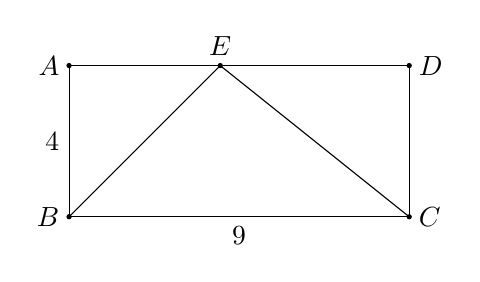
\begin{tikzpicture}[scale=0.48]
  \coordinate (A) at (0,4); \coordinate (B) at (0,0);
  \coordinate (C) at (9,0); \coordinate (D) at (9,4);
  \coordinate (E) at (4,4);
  \draw (A)--(B)--(C)--(D)--cycle;
  \draw (B)--(E)--(C);
  \foreach \p/\pos in {A/left,B/left,C/right,D/right,E/above}
    \fill (\p) circle(2pt) node[\pos]{$\p$};
  \node[left] at (0,2){$4$}; \node[below] at (4.5,0){$9$};
\end{tikzpicture}
\end{center}

  \answerarea[42mm]
\end{problem}


\needspace{8\baselineskip}

\begin{problem}[points=8]
  如图，在矩形 $ABCD$ 中，$AB=6$，$BC=8$。沿对角线 $AC$ 翻折，使点 $B$ 落在点 $B'$ 处，线段 $CB'$ 交 $AD$ 于点 $E$。求 $AE$ 的长。
\begin{center}
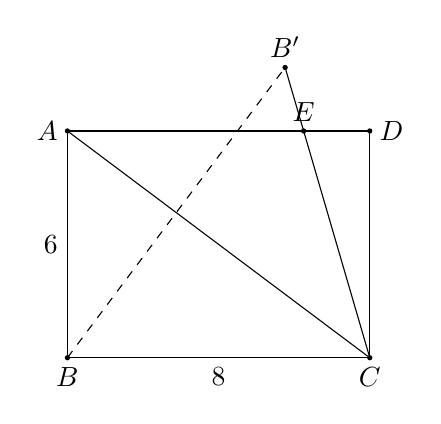
\begin{tikzpicture}[scale=0.48]
  \coordinate (A) at (0,6); \coordinate (B) at (0,0);
  \coordinate (C) at (8,0); \coordinate (D) at (8,6);
  \coordinate (E) at (6.25,6); \coordinate (Bp) at (5.76,7.68);
  \draw (A)--(B)--(C)--(D)--cycle;
  \draw (A)--(C);
  \draw[dashed] (B)--(Bp);
  \draw (C)--(Bp);
  \foreach \p/\pos in {A/left,B/below,C/below,D/right,E/above}
    \fill (\p) circle(2pt) node[\pos]{$\p$};
  \fill (Bp) circle(2pt) node[above]{$B'$};
  \node[left] at (0,3){$6$}; \node[below] at (4,0){$8$};
\end{tikzpicture}
\end{center}

  \answerarea[42mm]
\end{problem}


\needspace{8\baselineskip}

\begin{problem}[points=8]
  如图，在平行四边形 $ABCD$ 中，点 $E$ 在边 $CD$ 上，$CE=4$，$AE=6$。$AG$ 平分 $\angle BAE$，交 $CD$ 的延长线于点 $G$，且点 $G$ 在点 $C$ 的外侧。求 $CG$ 的长。
\begin{center}
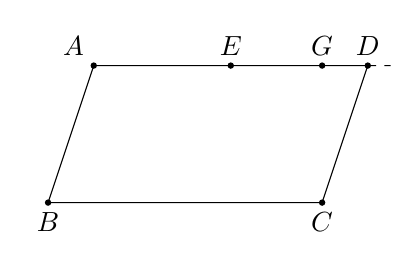
\begin{tikzpicture}[scale=0.58]
  \coordinate (A) at (0,3); \coordinate (B) at (-1,0);
  \coordinate (C) at (5,0); \coordinate (D) at (6,3);
  \coordinate (E) at (3,3); \coordinate (G) at (5,3);
  \draw (A)--(B)--(C)--(D)--cycle;
  \draw (A)--(E); \draw (A)--(G);
  \draw[dashed] (D)--(6.5,3);
  \foreach \p/\pos in {A/above left,B/below,C/below,D/above,E/above,G/above}
    \fill (\p) circle(2pt) node[\pos]{$\p$};
\end{tikzpicture}
\end{center}

  \answerarea[42mm]
\end{problem}


\needspace{8\baselineskip}

\begin{problem}[points=8]
  如图，在正方形 $ABCD$ 中，点 $E$ 是 $CD$ 的中点，$BF$ 平分 $\angle ABE$，交 $AD$ 于点 $F$。以点 $B$ 为原点，以 $BC$ 所在直线为 $x$ 轴，以 $BA$ 所在直线为 $y$ 轴建立平面直角坐标系。若点 $E$ 的坐标为 $(2,1)$，求点 $D$ 和点 $F$ 的坐标。
\begin{center}
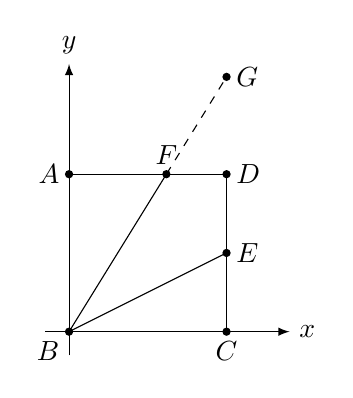
\begin{tikzpicture}[scale=1.0,>=latex]
  \draw[->] (-0.3,0)--(2.8,0) node[right]{$x$};
  \draw[->] (0,-0.3)--(0,3.4) node[above]{$y$};
  \coordinate (B) at (0,0); \coordinate (C) at (2,0);
  \coordinate (D) at (2,2); \coordinate (A) at (0,2);
  \coordinate (E) at (2,1); \coordinate (G) at (2,3.236);
  \coordinate (F) at (1.236,2);
  \draw (A)--(B)--(C)--(D)--cycle;
  \draw (B)--(E); \draw (B)--(F); \draw[dashed] (F)--(G);
  \foreach \p/\pos in {A/left,B/below left,C/below,D/right,E/right,F/above,G/right}
    \fill (\p) circle(1.5pt) node[\pos]{$\p$};
\end{tikzpicture}
\end{center}

  \answerarea[58mm]
\end{problem}



\end{document}
